% !TEX program = xelatex
\documentclass{article}
\usepackage{xeCJK}
\setCJKmainfont[
    BoldFont=cwTeXQHei-Bold,
    ItalicFont=cwTeXQYuan-Medium,
    Scale=1.1
]{cwTeXQFangsong-Medium}
\usepackage{/Users/jay/LaTeX/cs}
\usepackage{/Users/jay/LaTeX/codelist}

\renewcommand{\_}{\textscale{.5}{\textunderscore}}
\newcommand{\hmwkClass}{Operating System, Spring 2018}
\newcommand{\hmwkTitle}{Project 3}
\newcommand{\hmwkDueDate}{June 20, 2018}
\newcommand{\tb}{\textbf}

\begin{document}

\thispagestyle{empty}
\section*{\hmwkClass \\
    \normalsize{\hmwkTitle} \\
    \normalsize{DUE DATE: \hmwkDueDate}
}

\hfill{Team 16: \, B03505053 \, 曾彥青 \, B03902129 \, 陳鵬宇} \\

\subsection*{Code reading}

\begin{itemize}
    \item How readahead is called when page faults occur?
    \begin{itemize}
        \item mmap()
        \item filemap\_fault()
    \end{itemize}
\end{itemize}

The structure \tb{task\_struct} (defined in "linux/sched.h") contains a substructure \tb{mm\_struct} (defined in "linux/mm\_types.h") which is the memory descriptor, storing some useful information about the usage of memory. \\

In \tb{mm\_struct}, the first member is \tb{vm\_area\_struct}, the \textsl{memory region} (defined in "linux/mm\_types.h") which is a linked list of virtual memory area. \\

Thus we can get the following diagram:

\tikzstyle{block} = [rectangle, draw, text width=8em, text centered, rounded corners, minimum height=2em]
\tikzstyle{line} = [draw, -latex']
\begin{center}
\begin{tikzpicture}[node distance = 4cm, auto]
    % Place nodes
    \node [block] (a) {task\_struct};
    \node [block, right of=a] (b) {mm\_struct};
    \node [block, right of=b] (c) {vm\_area\_struct};
    \node [block, right of=c] (d) {fault};
    % Draw edges
    \path [line] (a) -- (b);
    \path [line] (b) -- (c);
    \path [line] (c) -- (d);
\end{tikzpicture}
\end{center}

In "linux/filemap.c", we can find following operations structure:

\begin{lstlisting}
const struct vm_operations_struct generic_file_vm_ops = {
    .fault		= filemap_fault,
};
\end{lstlisting}

Therefore, when a page fault occurs, it'll consequently invoke \tb{filemap\_fault()}, which will then check whether the required page is in the page cache by function \tb{find\_get\_page()} first.

There are two conditions:

\begin{enumerate}[label=(\alph*)]
    \item The page is in the page cache.
    \item The page is not in the page cache.
\end{enumerate}

For (a), we'll execute \tb{async\_readahead} to read pages.

For (b), we'll execute \tb{sync\_readahead} to read the required page and \textsl{readahead} other pages to cache. \\

Both \tb{do\_async\_mmap\_readahead()} and \tb{do\_sync\_mmap\_readahead()} will check whether VMA is randomly reading by \tb{VM\_RandomReadHint()}. 

If \tb{VM\_RandomReadHint()} returns true, it's no need to do \textsl{readahead}, therefore both functions will return; otherwise, both functions will keep executing.

Finally, we'll find the page by \tb{async\_readahead} and \tb{sync\_readahead} if \tb{MADV\_RANDOM} has no effect (VMA isn't reading randomly). If we found the page (checking by \tb{find\_get\_page()}), we'll lock the page and check whether it is truncated and up-to-date. After checking its size under page lock, we return the required page.

If \tb{MARD\_RANDOM} has no effect, we \text{goto} \tb{no\_cached\_page}, and it'll execute \tb{page\_cache\_read()} to read the required page and go back to \tb{find\_get\_page()}.

\subsection*{Revise the readahead algorithm for smaller response time}

We modify the original readahead function in "mm/readahead.c" and find that \tb{struct file\_ra\_state} defined in "include/linux/fs.h" controls the readahead state of the file.

We also change \tb{get\_next\_ra\_size()} to decide the size of readahead.

\begin{lstlisting}
static unsigned long get_next_ra_size(struct file_ra_state *ra, unsigned long max) {
    unsigned long cur = ra->size;
    unsigned long newsize;
    
    int ORIGINAL = false;
    
    if (ORIGINAL) {                 // original algorithm
        if (cur < max / 16)
            newsize = 4 * cur;
        else
            newsize = 2 * cur;
    } else {                        // revised algorithm
        if (cur < max / 32)
            newsize = 16 * cur;
        else if (cur < max / 16)
            newsize = 8 * cur;
        else
            newsize = 4 * cur;
    }

    return min(newsize, max);
}
\end{lstlisting}

There are two cases, and we test each case for 5 times:

\begin{enumerate}
    \item Original readahead.c

    $$
    \begin{array}{c|c|c|c|c|c|c}
        & 1 & 2 & 3 & 4 & 5 & average \\
        \hline
        \text{\# of major pagefault}    & 4158	& 4158	& 4158	& 4158	& 4158	& 4158 \\
        \text{\# of minor pagefault}    & 2639	& 2641	& 2640	& 2640	& 2641	& 2640.2 \\
        \text{\# of resident set size}  & 26620	& 26636 & 26624	& 26632	& 26632	& 26628.8 \\
        \hline
        \text{real}(sec) & 1.845 & 1.818 & 1.833 & 1.904  & 1.817 & 1.8434 \\ 
        \text{user}(sec) & 0	 & 0.036 & 0	 & 0.016  & 0	  & 0.0104 \\
        \text{sys}(sec)  & 0.018 & 0.16	 & 0.196 & 0.0192 & 0.176 & 0.11384
    \end{array}
    $$    

    \item Revised readahead.c

    $$
    \begin{array}{c|c|c|c|c|c|c}
        & 1 & 2 & 3 & 4 & 5 & average \\
        \hline
        \text{\# of major pagefault}    & 178	& 178	& 178	& 178	& 178	& 178 \\
        \text{\# of minor pagefault}    & 6618	& 6618	& 6619	& 6620	& 6620	& 6619 \\
        \text{\# of resident set size}  & 26476 & 26476 & 26476 & 26476 & 26476 & 26476 \\
        \hline
        \text{real}(sec) & 0.35	 & 0.371 & 0.378 & 0.359 & 0.354 & 0.3624 \\ 
        \text{user}(sec) & 0	 & 0	 & 0.012 & 0.012 & 0.004 & 0.0056 \\
        \text{sys}(sec)  & 0.064 & 0.064 & 0.06	 & 0.06	 & 0.068 & 0.0632
    \end{array}
    $$    

\end{enumerate}

\newpage
\subsection*{Screenshots}

\begin{figure}[!htb]
    \centering
    \begin{subfigure}[b]{0.49\textwidth}
        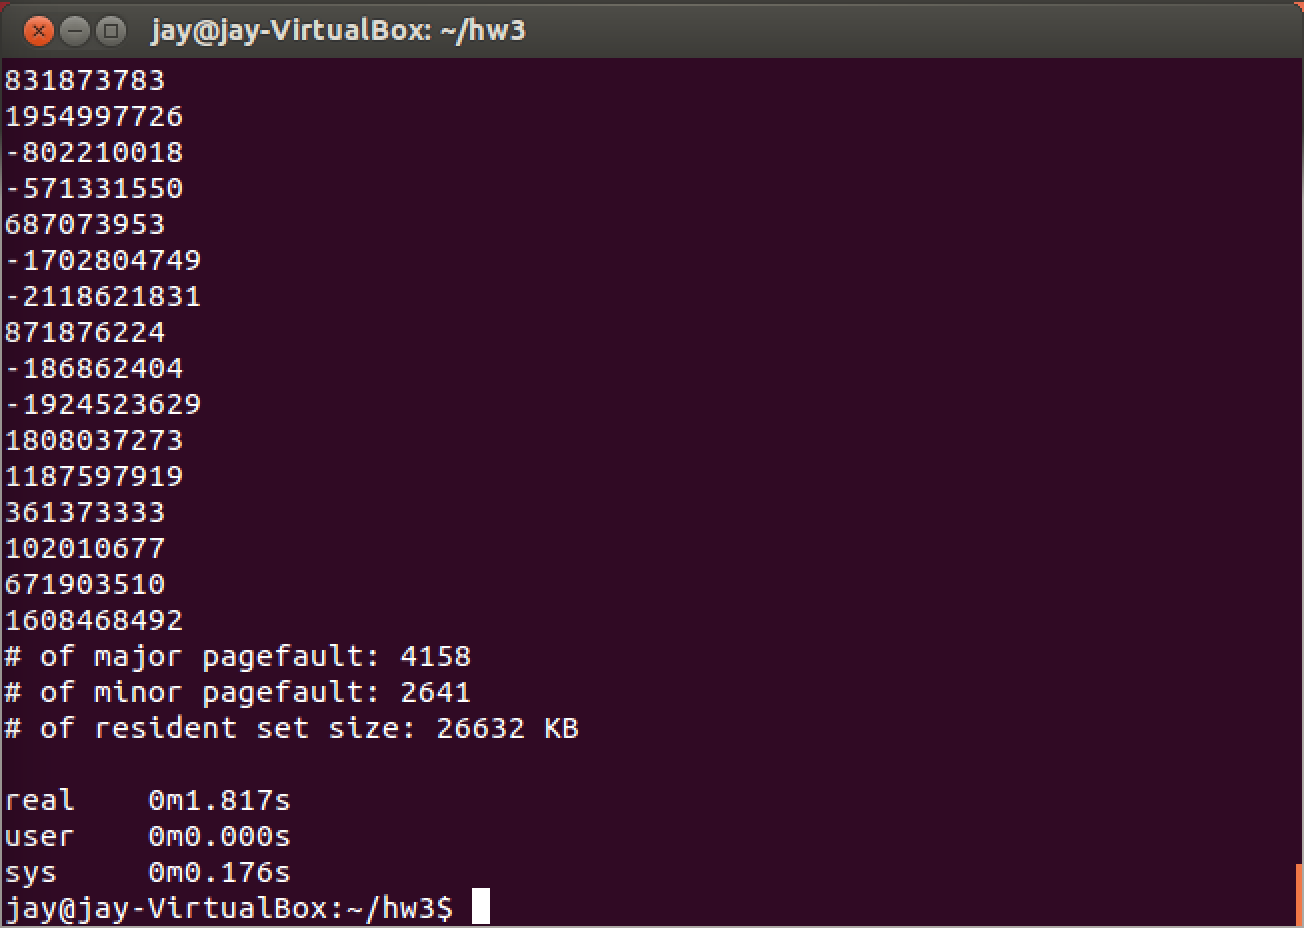
\includegraphics[width=\textwidth]{img/128.png}
        \caption{Original algorithm}
    \end{subfigure}
    ~
    \begin{subfigure}[b]{0.49\textwidth}
        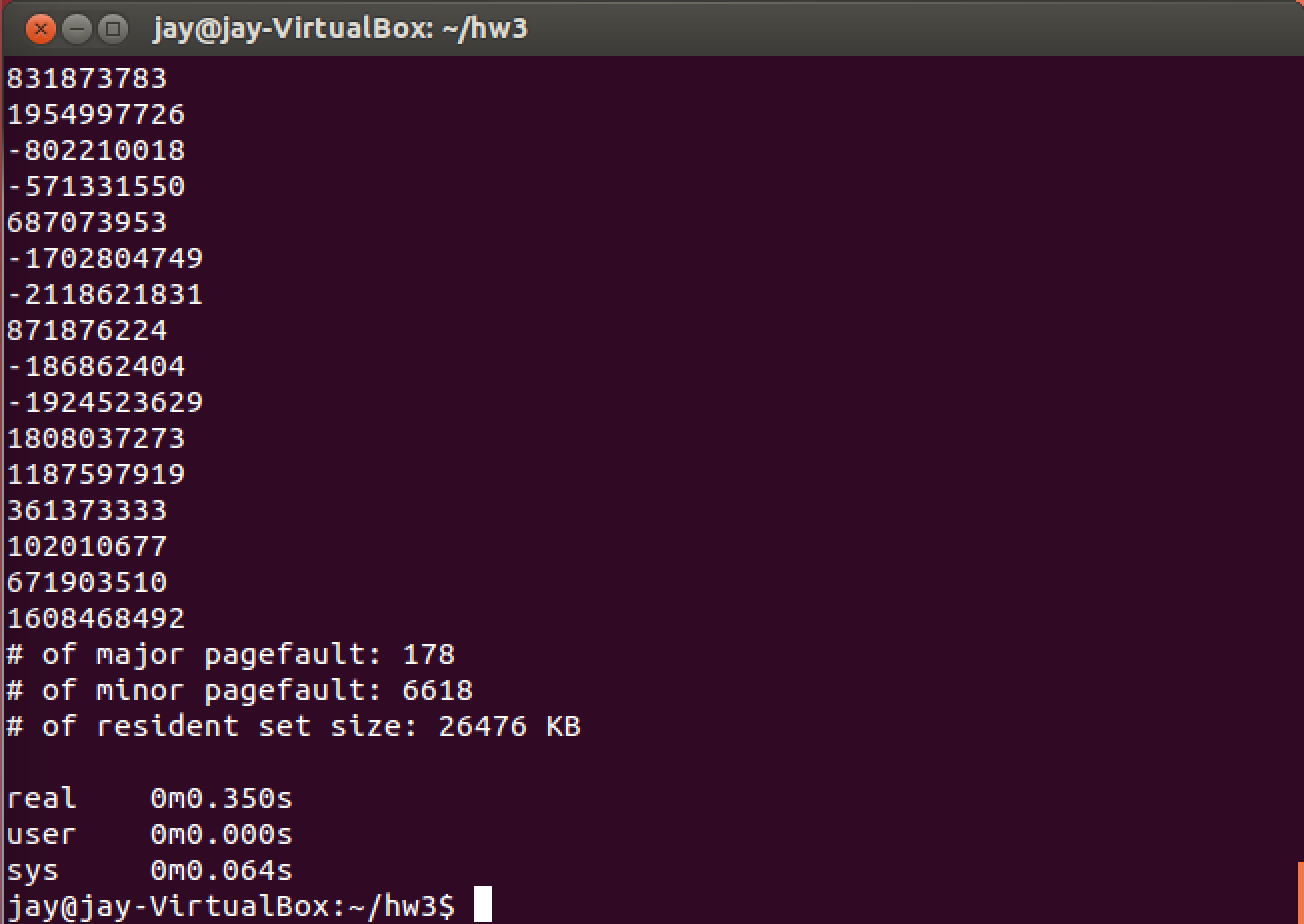
\includegraphics[width=\textwidth]{img/2048.png}
        \caption{Revised algorithm}
    \end{subfigure}
\end{figure}

\begin{figure}[!htb]
    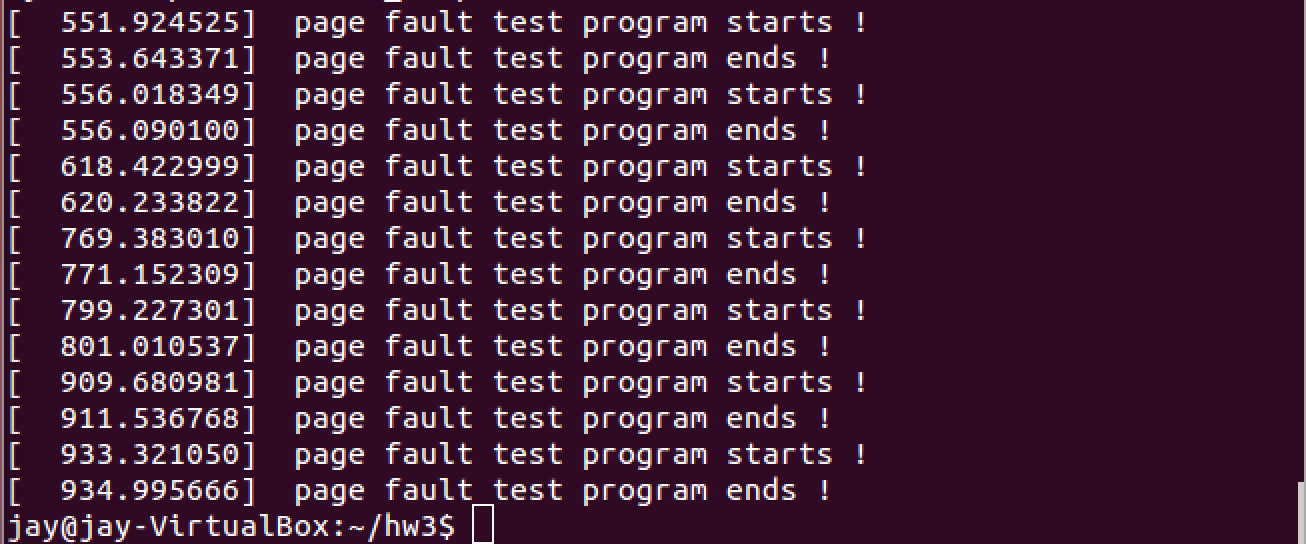
\includegraphics[width=\textwidth]{img/test.png}
\end{figure}

\newpage
\subsection*{Bonus}

We use the following command to change the size of \tb{VM\_MAX\_READHEAD} and test the revised algorithm, and we don't revise any code.

\begin{lstlisting}
  $ sudo /sbin/blockdev --setra 512 /dev/sda
  $ sudo /sbin/blockdev --setra 2048 /dev/sda
  $ sudo /sbin/blockdev --setra 8192 /dev/sda
\end{lstlisting}

Different size of \tb{VM\_MAX\_READHEAD}:

$$
\begin{array}{c|c|c|c|c}
    & 128 \text{(original)} & 512 & 2048 & 8192 \\
    \hline
    \text{average time}(sec) & 1.8434 & 1.593 & 0.3624 & 0.281
\end{array}
$$

\subsubsection*{Screenshots}

\begin{figure}[!htb]
    \centering
    \begin{subfigure}[b]{0.49\textwidth}
        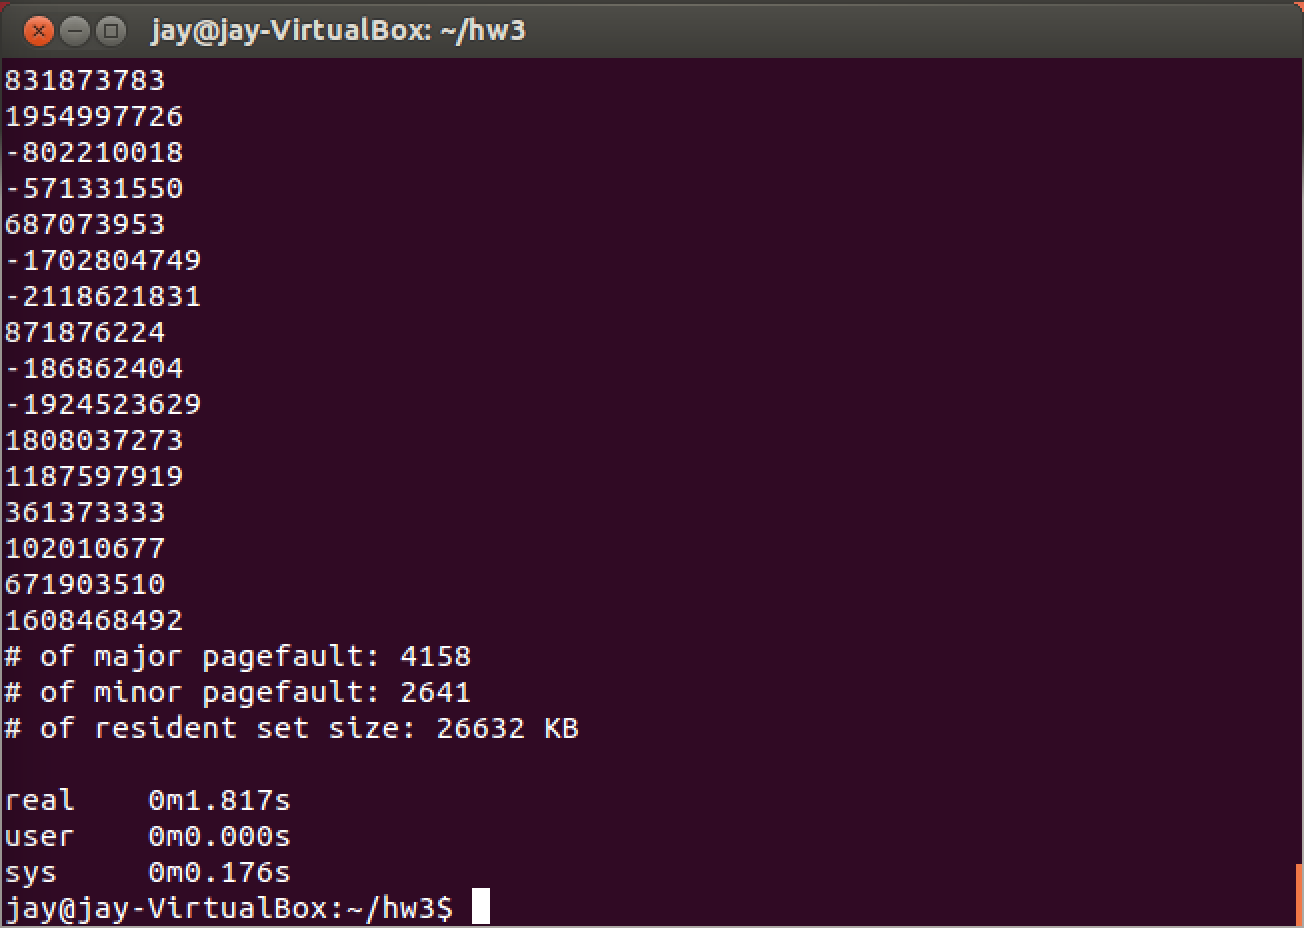
\includegraphics[width=\textwidth]{img/128.png}
        \caption{VM\_MAX\_READHEAD = 128}
    \end{subfigure}
    ~
    \begin{subfigure}[b]{0.49\textwidth}
        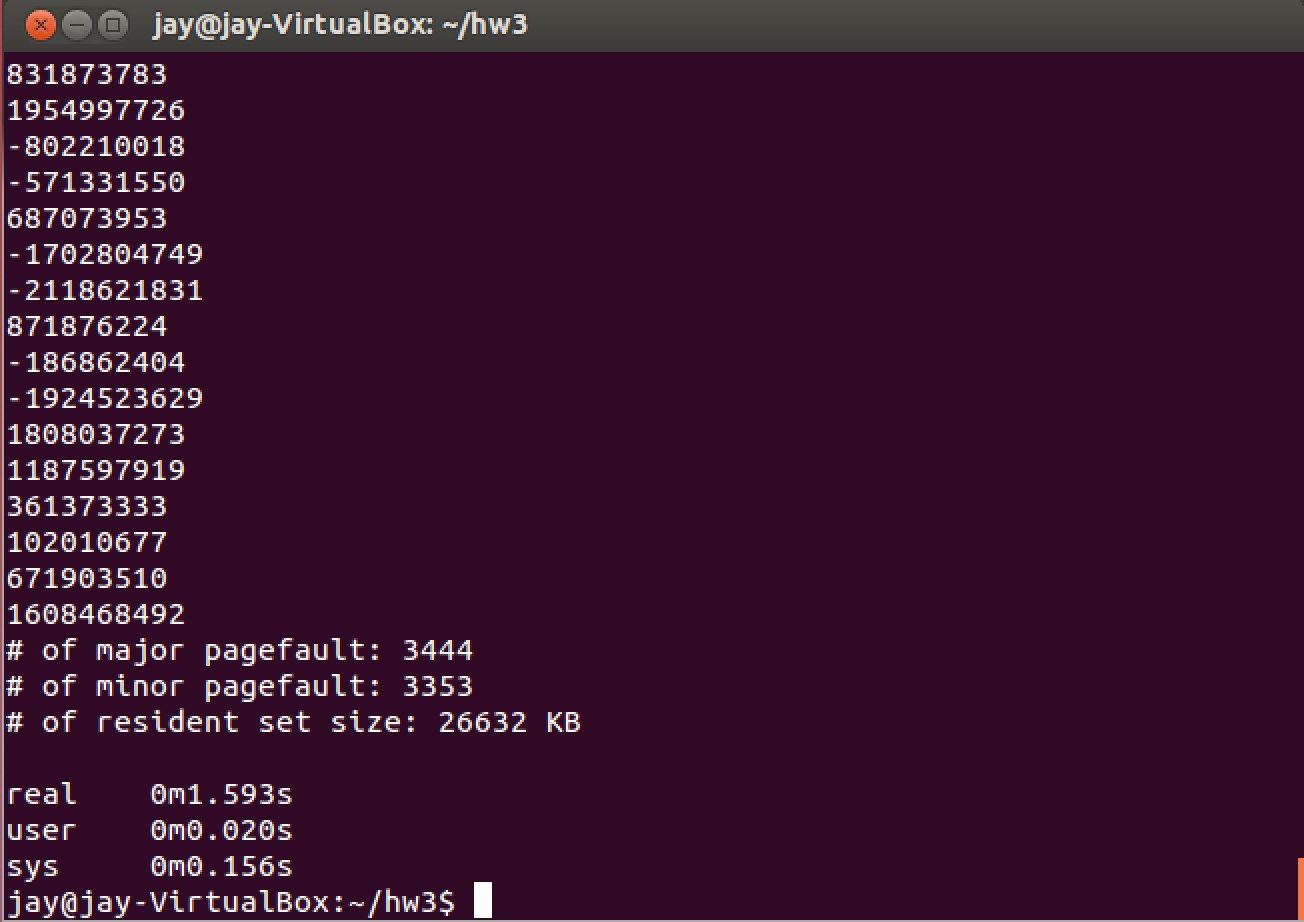
\includegraphics[width=\textwidth]{img/512.png}
        \caption{VM\_MAX\_READHEAD = 512}
    \end{subfigure}
    ~
    \begin{subfigure}[b]{0.49\textwidth}
        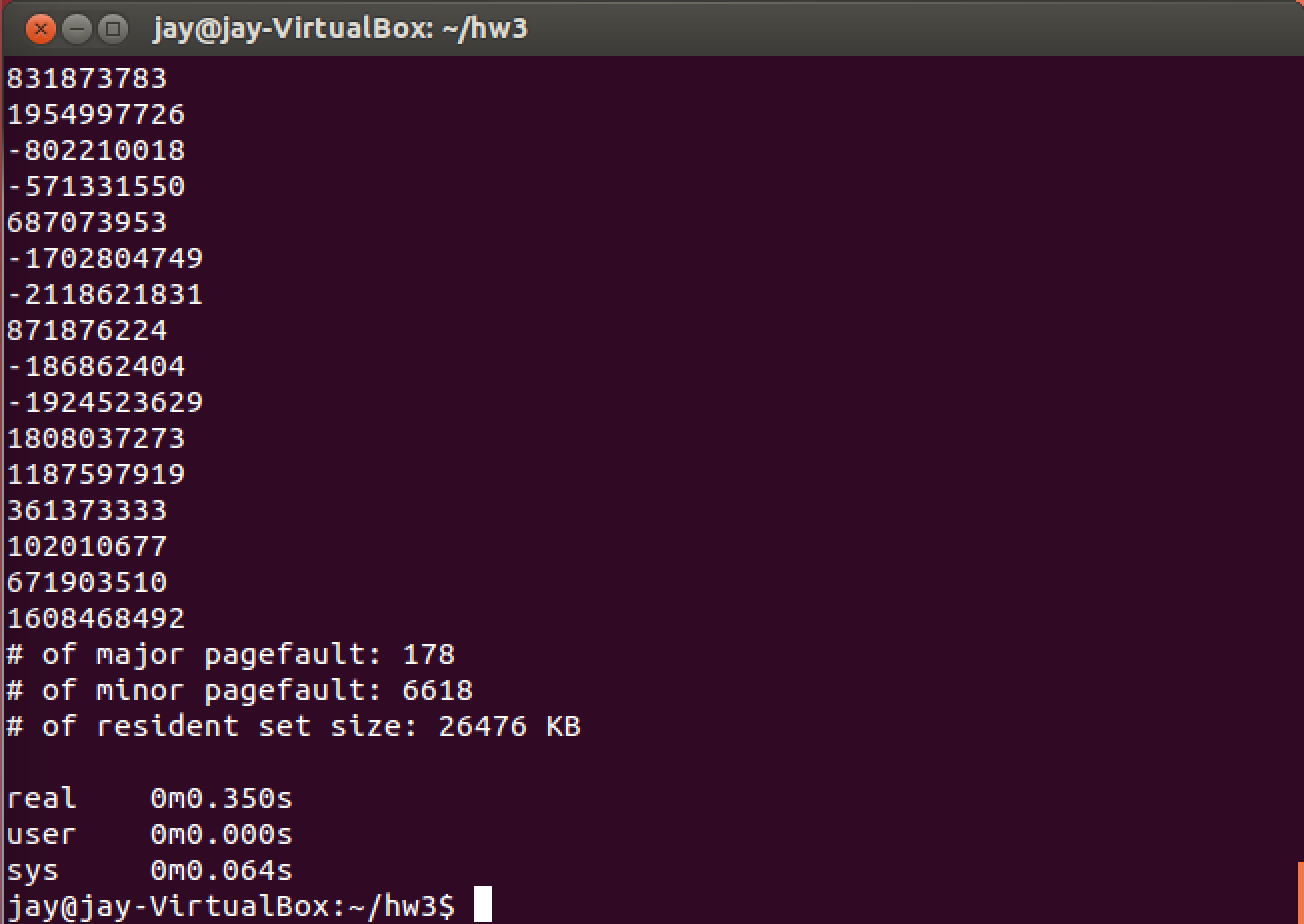
\includegraphics[width=\textwidth]{img/2048.png}
        \caption{VM\_MAX\_READHEAD = 2048}
    \end{subfigure}
    ~
    \begin{subfigure}[b]{0.49\textwidth}
        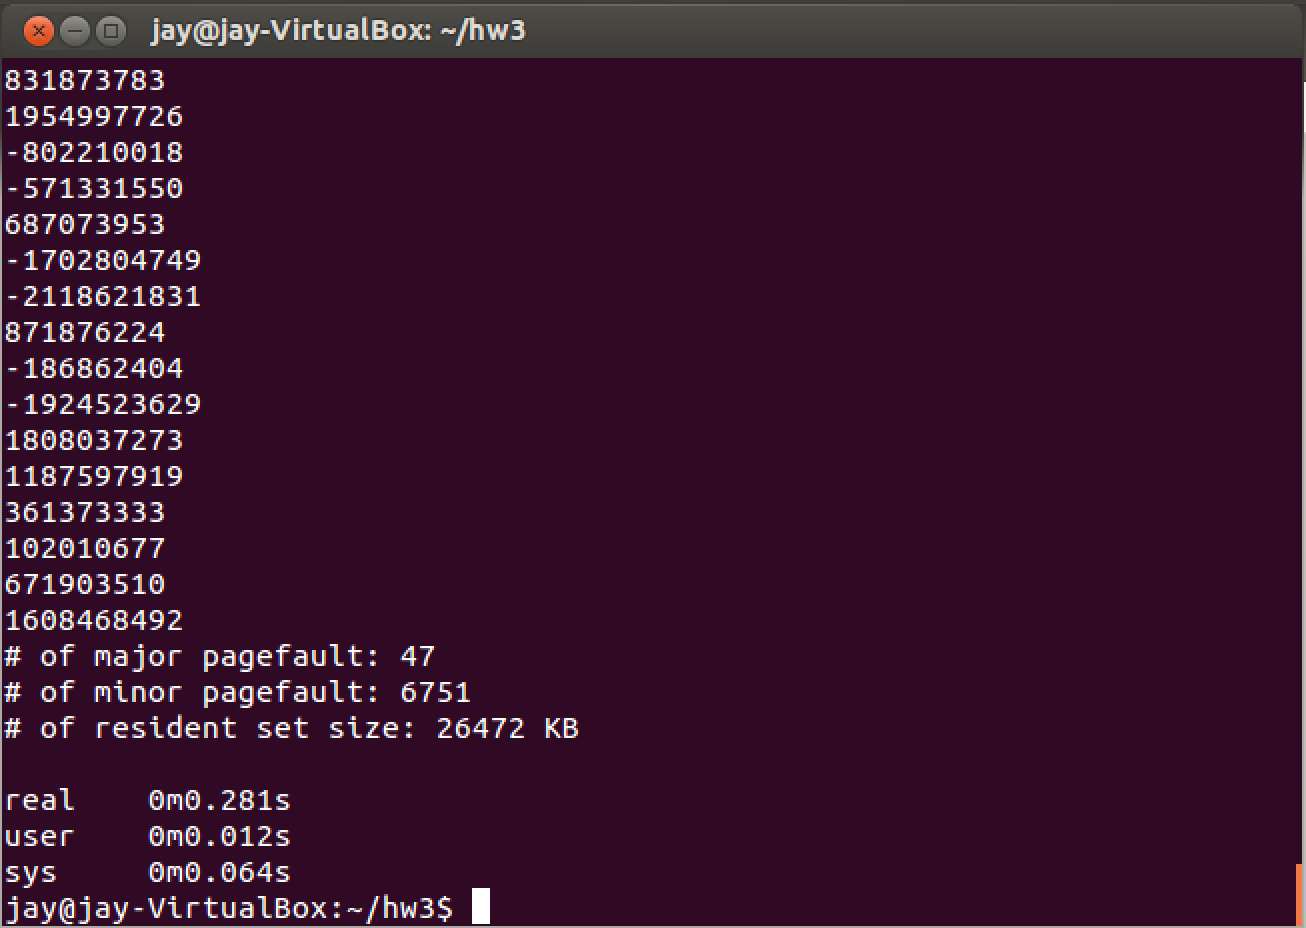
\includegraphics[width=\textwidth]{img/8192.png}
        \caption{VM\_MAX\_READHEAD = 8192}
    \end{subfigure}
\end{figure}

It's obvious that after enlarging \tb{VM\_MAX\_READHEAD}, the real time is reduced. The reason is that when the parameter is enlarged, it'll make the number of pages we can pre-read each time more, thus letting the times of major page fault lesser, and improving the efficiency.

\end{document}